%%
%% Copyright 2007-2020 Elsevier Ltd
%%
%% This file is part of the 'Elsarticle Bundle'.
%% ---------------------------------------------
%%
%% It may be distributed under the conditions of the LaTeX Project Public
%% License, either version 1.2 of this license or (at your option) any
%% later version.  The latest version of this license is in
%%    http://www.latex-project.org/lppl.txt
%% and version 1.2 or later is part of all distributions of LaTeX
%% version 1999/12/01 or later.
%%
%% The list of all files belonging to the 'Elsarticle Bundle' is
%% given in the file `manifest.txt'.
%%
%% Template article for Elsevier's document class `elsarticle'
%% with harvard style bibliographic references

%\documentclass[preprint,12pt,authoryear]{elsarticle}

%% Use the option review to obtain double line spacing
%% \documentclass[authoryear,preprint,review,12pt]{elsarticle}

%% Use the options 1p,twocolumn; 3p; 3p,twocolumn; 5p; or 5p,twocolumn
%% for a journal layout:
%% \documentclass[final,1p,times,authoryear]{elsarticle}
%% \documentclass[final,1p,times,twocolumn,authoryear]{elsarticle}
%% \documentclass[final,3p,times,authoryear]{elsarticle}
%% \documentclass[final,3p,times,twocolumn,authoryear]{elsarticle}
%% \documentclass[final,5p,times,authoryear]{elsarticle}
 \documentclass[final,5p,times,twocolumn,authoryear]{elsarticle}

%% For including figures, graphicx.sty has been loaded in
%% elsarticle.cls. If you prefer to use the old commands
%% please give \usepackage{epsfig}

%% The amssymb package provides various useful mathematical symbols
\usepackage{amssymb}
%% The amsthm package provides extended theorem environments
%% \usepackage{amsthm}

%% The lineno packages adds line numbers. Start line numbering with
%% \begin{linenumbers}, end it with \end{linenumbers}. Or switch it on
%% for the whole article with \linenumbers.
%% \usepackage{lineno}


\begin{document}

\begin{frontmatter}

\title{WE NEED A TITLE HEERE ???}

\author[first]{Leonor Ramos}
\author[second]{Tiago Patrício}
\author[third]{João Almeida}
\author[fourth]{David Mendes}
\affiliation{organization={ISCTE – Instituto Universitário de Lisboa}, country={Portugal}} % Title page setup

\begin{abstract}
%% Text of abstract
This article aims to summarize the approach and results of \cite{Stacking}, in which the authors explore employing stacking, boosting, and blending machine learning algorithms to predict student performance in large-scale assessments based on a wide range of predictors and compare their performance.
\end{abstract}

\begin{keyword}
PISA \sep Machine learning \sep Stacking \sep Boosting \sep Blending \sep Ensemble
learning
\end{keyword}

\end{frontmatter}

%\tableofcontents

%% \linenumbers

%% main text

\section{Introduction}
\label{introduction}

The study \cite{Stacking} uses the PISA 2022 Student questionnaire dataset, focusing on student responses and performance in subjects of mathematics, reading, and science. The authors employ machine learning algorithms to predict student performance, including stacking, blending, and boosting algorithms. The stacking method combines predictions from multiple models to create a meta-model that improves overall prediction performance. Boosting algorithms sequentially train models, each correcting errors from the previous ones, while blending uses a validation set to train the base learners. This study aims to measure the prediction performance of these methods.
\section{Methods}
%%\label{}

\subsection{Stacking}
Stacking is an ensemble learning technique developed by \cite{WOLPERT1992241} that combines several prediction models and uses their outputs as input for a next-level model (meta-model), aiming to improve overall prediction performance\cite{Stacking}. In the study \cite{Stacking}, the authors divide stacking into level 0 and level 1, where layer 0 refers to where the different models generate distinct predictions, and level 1 combines predictions of level 0. For level 0, some of the different models that could be used are DTs, NNs, SVMs, and kNN, in which the resulting predictions are then used and combined in layer 1, in order to improve the overall prediction \cite{WOLPERT1992241}, the authors choose to use ridge regression, which can be useful to avoid overfitting \cite{CUI2021107038}
\subsection{Boosting}
Because the dataset used in this study is composed of missing data, it is imperative to implement learners that deal with missing data, the boosting algorithms used were XGBoost, HGB, and LightGBM \cite{Stacking}
\subsection{blending}
Blending and stacking are both techniques used in ensemble learning that share similarities. The key difference between them is that in blending, the base learners are trained using predictions obtained from the validation set instead of directly from the training set\cite{Stacking}
\section{Results}
The study found that the stacking method produced the lowest error metrics (Mean Absolute Percentage Error (MAPE), Mean Absolute Error (MAE), Mean Squared Error (MSE)) for most countries compared to boosting and blending. Robust linear mixed-effects models indicated that stacking had significantly lower error metrics across all subjects as showed in \ref{fig:results}.

\begin{figure}
	\centering
	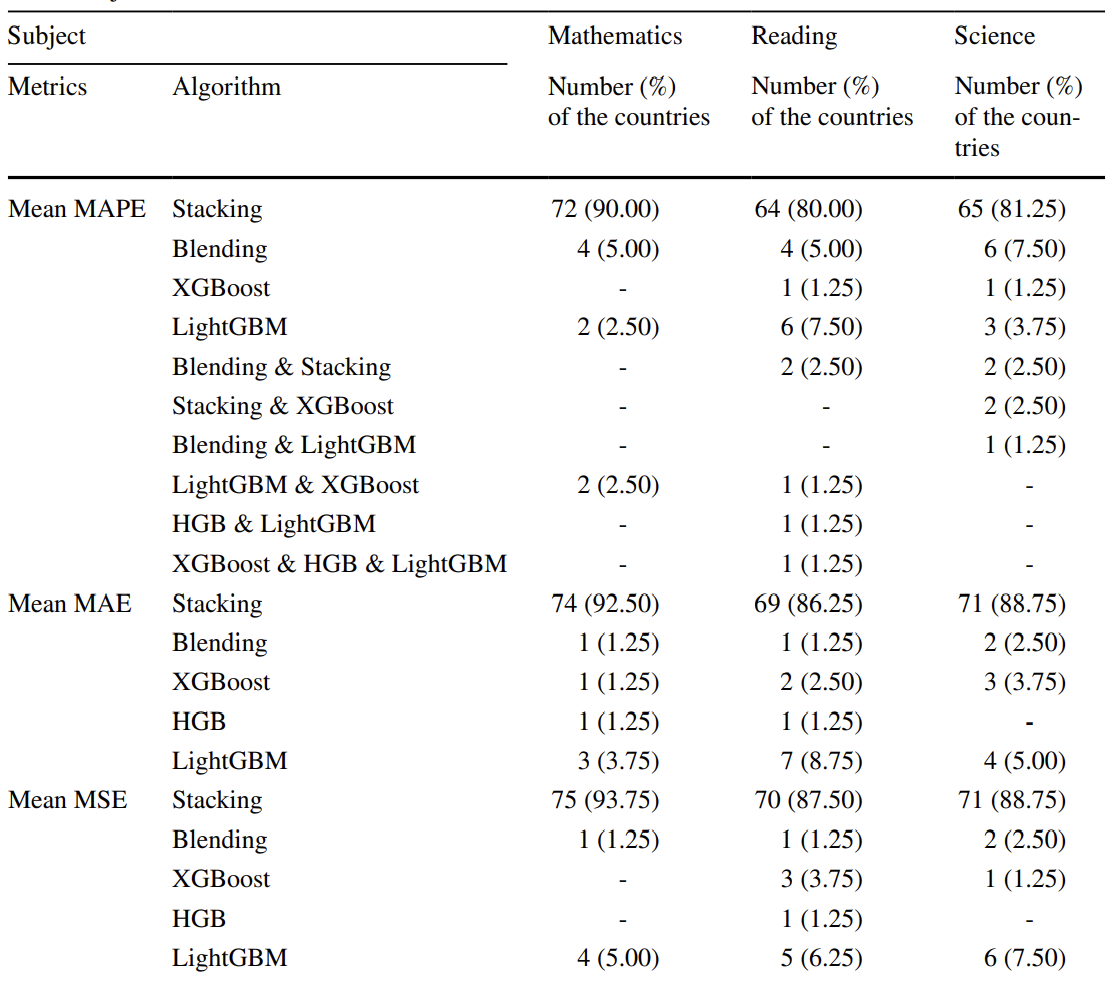
\includegraphics[width=0.4\textwidth]{figures/figure1}
	\caption{The Number (\%) of the countries exhibiting the lowest error values generated by each algorithm for all subjects \cite{Stacking}}
    \label{fig:results}
\end{figure}

\section{Conclusion}
The study \cite{Stacking} concludes that stacking is a favorable option for better performance, stable and accurate predictions based on evaluation with various metrics such as MAPE, MAE, MSE and RMSE where it obtained a significant metric score in all subjects compared to boosting and blending.
Due to this study only evaluating the PISA dataset, I think it would be interesting to evaluate it with other datasets to improve this analysis further


%% If you have bibdatabase file and want bibtex to generate the
%% bibitems, please use
%%
\bibliographystyle{elsarticle-harv}
\bibliography{main}

%% else use the following coding to input the bibitems directly in the
%% TeX file.

%%\begin{thebibliography}{00}

%% \bibitem[Author(year)]{label}
%% For example:

%% \bibitem[Aladro et al.(2015)]{Aladro15} Aladro, R., Martín, S., Riquelme, D., et al. 2015, \aas, 579, A101


%%\end{thebibliography}

\end{document}

\endinput
%%
%% End of file `elsarticle-template-harv.tex'.
